% !TEX root = DesignDocument.tex


\chapter{Testing}
\label{ch:testing}

% This section describes the approach taken with regard to system and unit testing.    This chapter does not describe the outcome of those tests.    

\section{Overview}
The testing approach is based on manual testing so far. 
The website and file conversion are tested separately, with their integration being tested as well.
Our tests ensure that the features provided in our user stories are met and work as intended.
The tests for each user story can be found below.

\section{Dependencies}
The main testing framework for the Azure website is Microsoft's C\# testing framework. 
The file conversion needs no external testing framework as it is tested manually for accuracy.

\section{Test design and setup}
There are currently no unit tests for the website, as all testing has been done by hand so far.
We may utilize Microsoft's C\# testing framework in the future. There is currently a testing project setup for the website but there are no tests currently available in it.
The file conversion testing is performed manually, as we cannot validate accuracy of conversion through software alone. We have a variety of files that we have tested through our development that we've used to show we can convert from one format to another.

\begin{itemize} \item Upload Maple 3D file to a cloud server \end{itemize}
\hspace{7mm}    
    Tested by manually accessing the website and uploading a file, then checking that it is present in the filesystem.

\begin{itemize} \item Maple 3D file will be automatically converted to a QR tag \end{itemize}
    \hspace{7mm}
    This feature is not yet implemented, but the conversion test was tested manually as a part and the as a system with the website.

\begin{itemize} \item Download the QR tag for a model from the cloud server \end{itemize}
    \hspace{7mm}
    Tags for models are not yet available, but a user can download a converted version of their uploaded file.

\begin{itemize} \item View the QR tag with an AR headset and render the 3D model \end{itemize}
    \hspace{7mm} 
    QR tags are not yet implemented, but we successfully rendered 3D models on the hololens by accessing files through OneDrive or using the converted file from the upload page.

\begin{itemize} \item Convert a 3D file from one format to another 
    \end{itemize}
    \hspace{7mm}
    The file conversion is manually tested using a variety of inputs to ensure robust and consistent performance. As there are two libraries (assimp and FBX SDK), they were both manually tested for simple functionality as the were implemented. After the two were put together, we had more tests to run. We tried sending through file types that can be inputs for assimp and made sure that the file made it to the FBX section and output the correct file format (.fbx). There are many different inputs so we sent through files for the common types we would expect such as .stl, .obj, .dae etc. Unsupported file types were also tested and we received appropriate errors from the conversion libraries. The file types supported for our system are available in Table \ref{tab:suportedfiletypes}. We also tried large files so we would know how long we could expect the system to take to process files of different sizes. There are certain limitations on the HoloLens hardware for file size and complexity that can be rendered, so we are aware of the limitations on that end and will inform our users appropriately. 
    
    We also tested files with textures embedded in them, to make sure the textures get converted with the file. With the file types we tried such as .obj and .fbx, the textures converted with the files as expected. The default 3d file viewer in the HoloLens currently does not support colors or textures, so we have not been able to test these features on the HoloLens yet. 

    The test files we ran through our system came from a variety of sources. We had a simple sphere generated in Maple as a .stl file, which we successfully converted through our system to .fbx to view on the HoloLens. We also received a .fbx representing a column, sent to us from a mathematics professor. The website \url{http://free3d.com} has many 3d files of varying formats and we ran some of them through our system. Sample files included a car, building, space ship, Batman, and other unique files. These files were available as .fbx and were good for testing out the HoloLens, but usually other formats came with them that we could convert them to .fbx as well. Lastly, we received some sample architectural files from one student's family member that were drawings of large buildings in .fbx format. One of these files rendered in the HoloLens, but the other two were too large to render because they exceeded the mesh/vertex limit for the viewer. This was when we looked into the limitations of the built in viewer.

    An example of converting a file through our system can be seen below in Figures \ref{Car-FBX}, \ref{Car-OBJ}, and \ref{Car-STL}. 
    We found a 3d file for a car online in the FBX format. 
    Our system then converted it to an OBJ format, as the File Converter software determined it only needed the FBX SDK to convert from FBX $\rightarrow$ OBJ. 
    The third model is an STL file generated from the FBX file, using a DAE file as an intermediate format between the FBX SDK and assimp libraries. 
    As is apparent in Figure \ref{Car-STL} below, the STL file does not contain the colors or smooth surfaces that are present in the other file types, and this is a limitation of the STL file format. 
    This system works for converting STL $\rightarrow$ FBX as well, but the colors would not be present in the final file because that information is not contained in the STL. 
    The STL format is one that can be exported from Maple software.

\begin{itemize} \item All other user stories post MVP are not yet implemented or tested, and they pertain mostly to secure accounts, file permissions, and more advanced features on the HoloLens viewer. 
These features will be tested appropriately through manual testing or the C\# framework as they are developed. \end{itemize}

\begin{figure}[H]
    \centering
    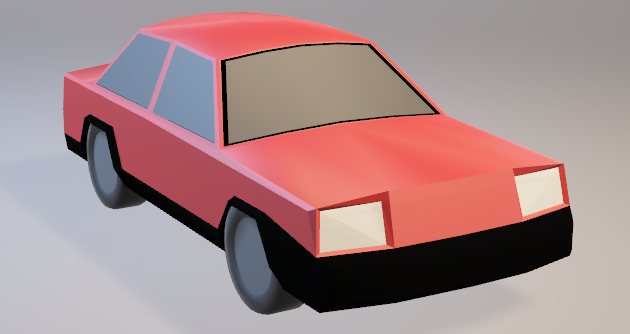
\includegraphics[width=\textwidth]{Car-FBX.png}
    \caption{Car FBX File}
    \label{Car-FBX}
\end{figure}

\begin{figure}[H]
    \centering
    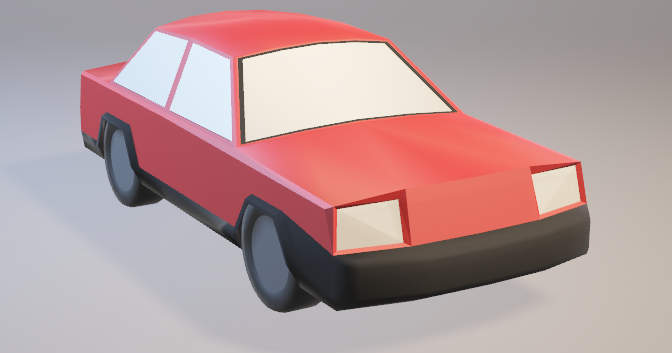
\includegraphics[width=\textwidth]{Car-OBJ.png}
    \caption{Car OBJ File}
    \label{Car-OBJ}
\end{figure}

\begin{figure}[H]
    \centering
    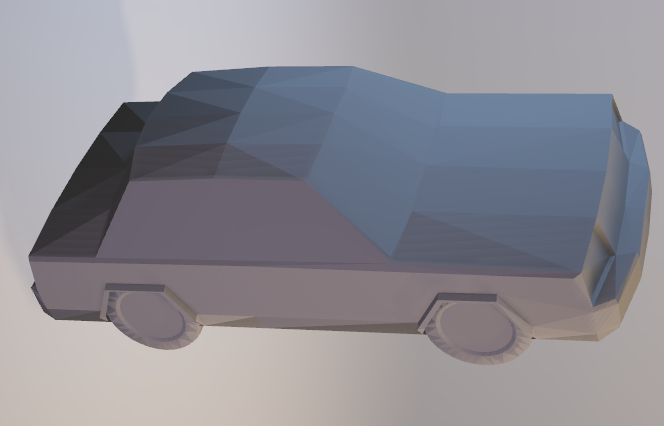
\includegraphics[width=\textwidth]{Car-STL.png}
    \caption{Car STL File}
    \label{Car-STL}
\end{figure}

\section{System Testing}
Testing our system involved manually using our software as a user would.
The test relied on being able to access the website, uploading a file, and being able to download the converted version of it.
This was successfully tested through manual tests and these features were present in our MVP.

\section{System Integration Analysis}
We performed some manual tests while integrating the file conversion with the website.
The integration was relatively simple and required us only to upload the executable to Azure and call it as we regularly would from our PC.
We successfully uploaded, converted, and downloaded files using the website to access the file conversion software.

\section{Risk Analysis}
There are two main risks associated with our project. These risks pertain to the functionality of the product itself and the security of our data.
Minimizing and preventing these risks are vital to providing quality software and positive relationships with users.

The first risk is that the software may fail to convert or render a given input file.
This could be caused by the file being too large or complex for our system to handle, or part of the file is corrupt. 

File security poses the other risk to our project, as some of the files uploaded may contain sensitive or confidential data.
We want to ensure that we maintain our users' privacy and trust as we strive to ensure only specified people can access certain files.
\subsection{Risk Mitigation}
To mitigate these risks, we have multiple strategies implemented to prevent the issues from happening in the first place.

Addressing the first risk of failed conversion or rendering, we will ensure product quality through rapid iteration and testing of MVPs. 
We have a variety of test files of varying sizes and formats that we have run through our system to make sure we cover many of the common (and uncommon) use cases.
Additionally, we aim to stay informed on the documentation of the libraries and platforms we use in our software to make sure we understand the capabilities and limitations of the tools we are using.
Especially for the file conversion software, we have researched which file types can be run through the libraries and have implemented that functionality in our product and need to communicate to our users which file types are acceptable for our system. 

For the second risk of data security, we try our best to examine and remove any possible security holes in our data flow.
We will need to analyze the website code to limit file access only to properly-privileged users. 
We also plan to implement features such as https and end-to-end encryption to maintain data security on our connections.


\section{Mobile Testing}
    Testing for the mobile app was primarily done manually. This is because most testing was done on visualizing files and verifying the app performed as expected.  It was also verifying that HTTP packets were as expected going to and from the phone.

    When error messages are printed to the user of the app, a toast is displayed.  A toast is the small box that pops up on the lower section of the screen.

    \subsection{Files}
        A variety of files were used throughout development to test functionality of the app. Some sample files were found on \url{https://free3d.com}. Some files were provided from Dr. Deschamp and others were generated in Maple. Different files were used to test that colors were working both in the MTL and as PNGs. Additionally, large and small files were tested to see how the app reacted to more complex files. The BMW file seen below is an example of a complex file that doesn't render well in the app and demonstrates the limitations of the app.
        
        \subsubsection{Colors}
        
            A major feature requested for the app was to be able to display colors. The example below shows a simple sphere with a proof of concept that colors do work. The car is a more in-depth example that shows multiple colors on the same model.
            
            \begin{figure}[H]
                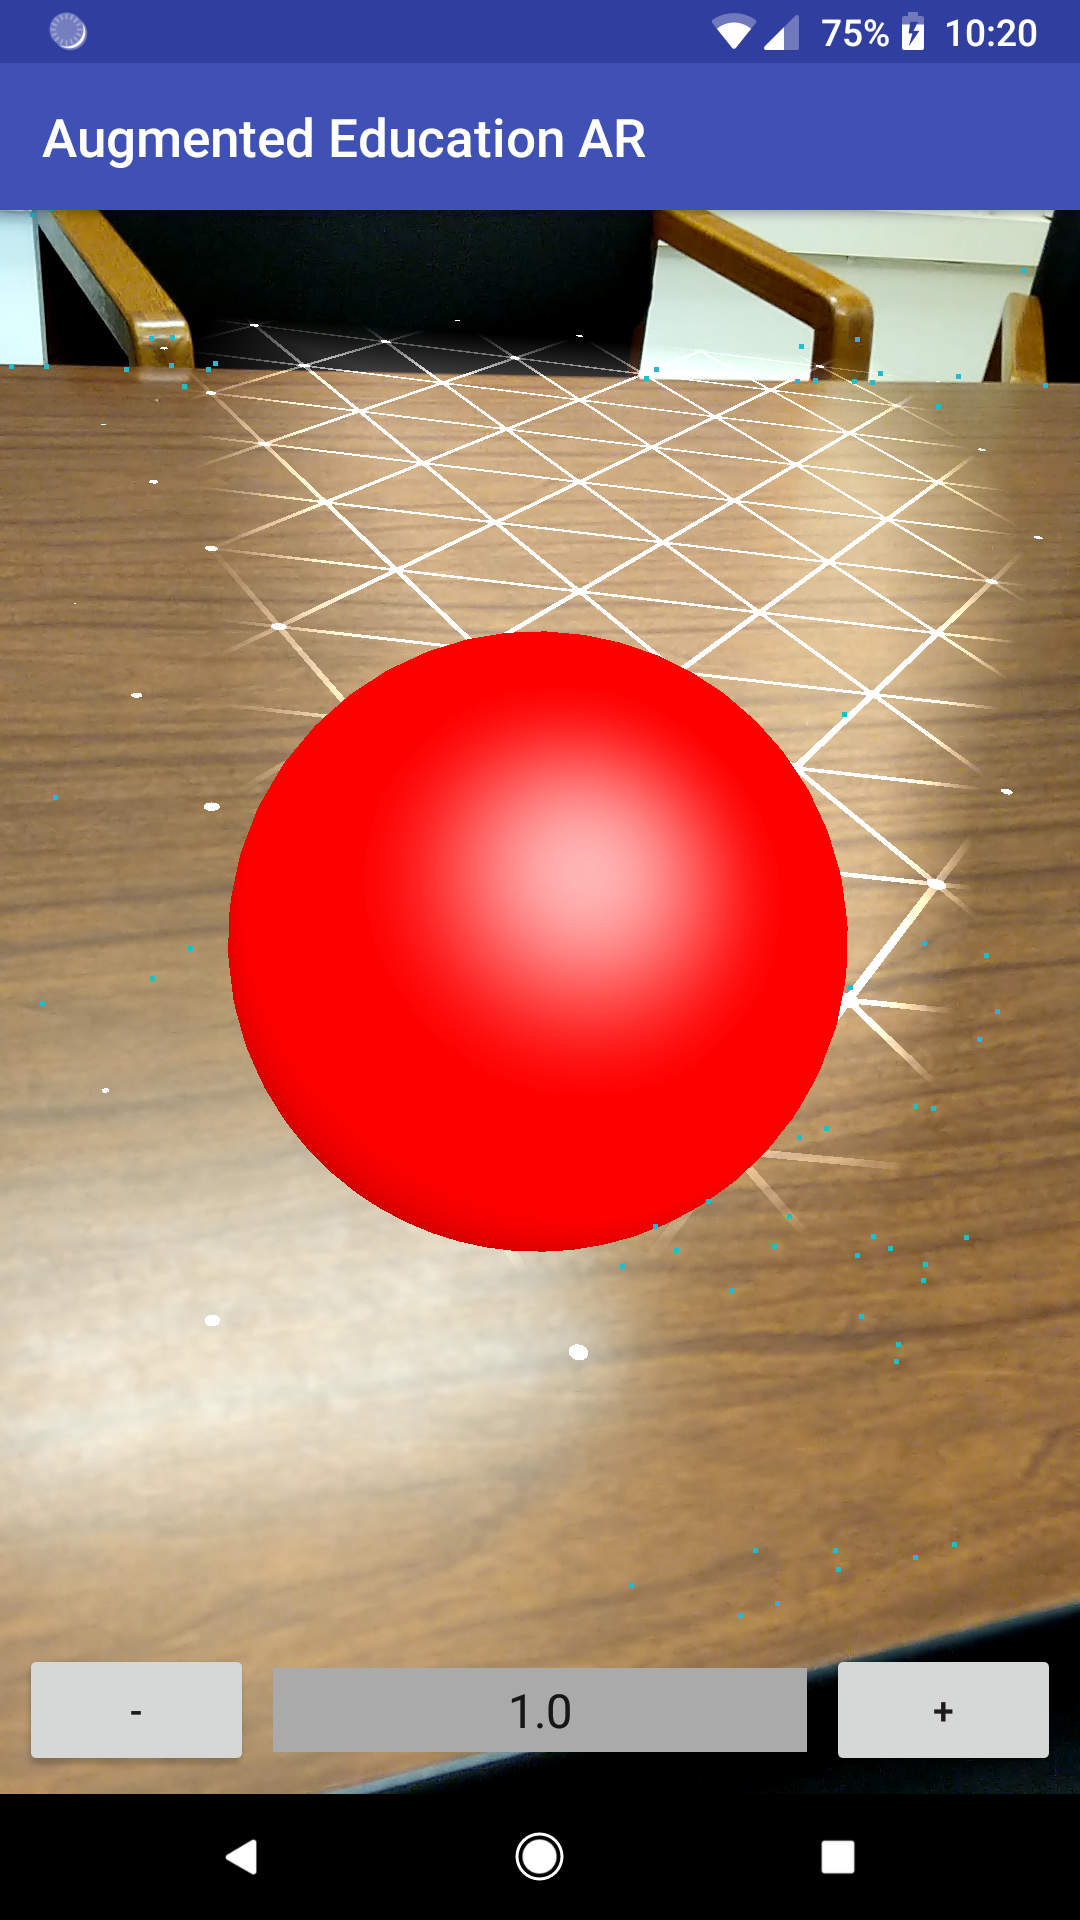
\includegraphics[width=0.5\textwidth]{Mobile/Mobile_RedSphere}
                \centering
                \caption{Colors - Red Sphere}
                \label{fig:mobileRedSphere}
            \end{figure}

            \begin{figure}[H]
                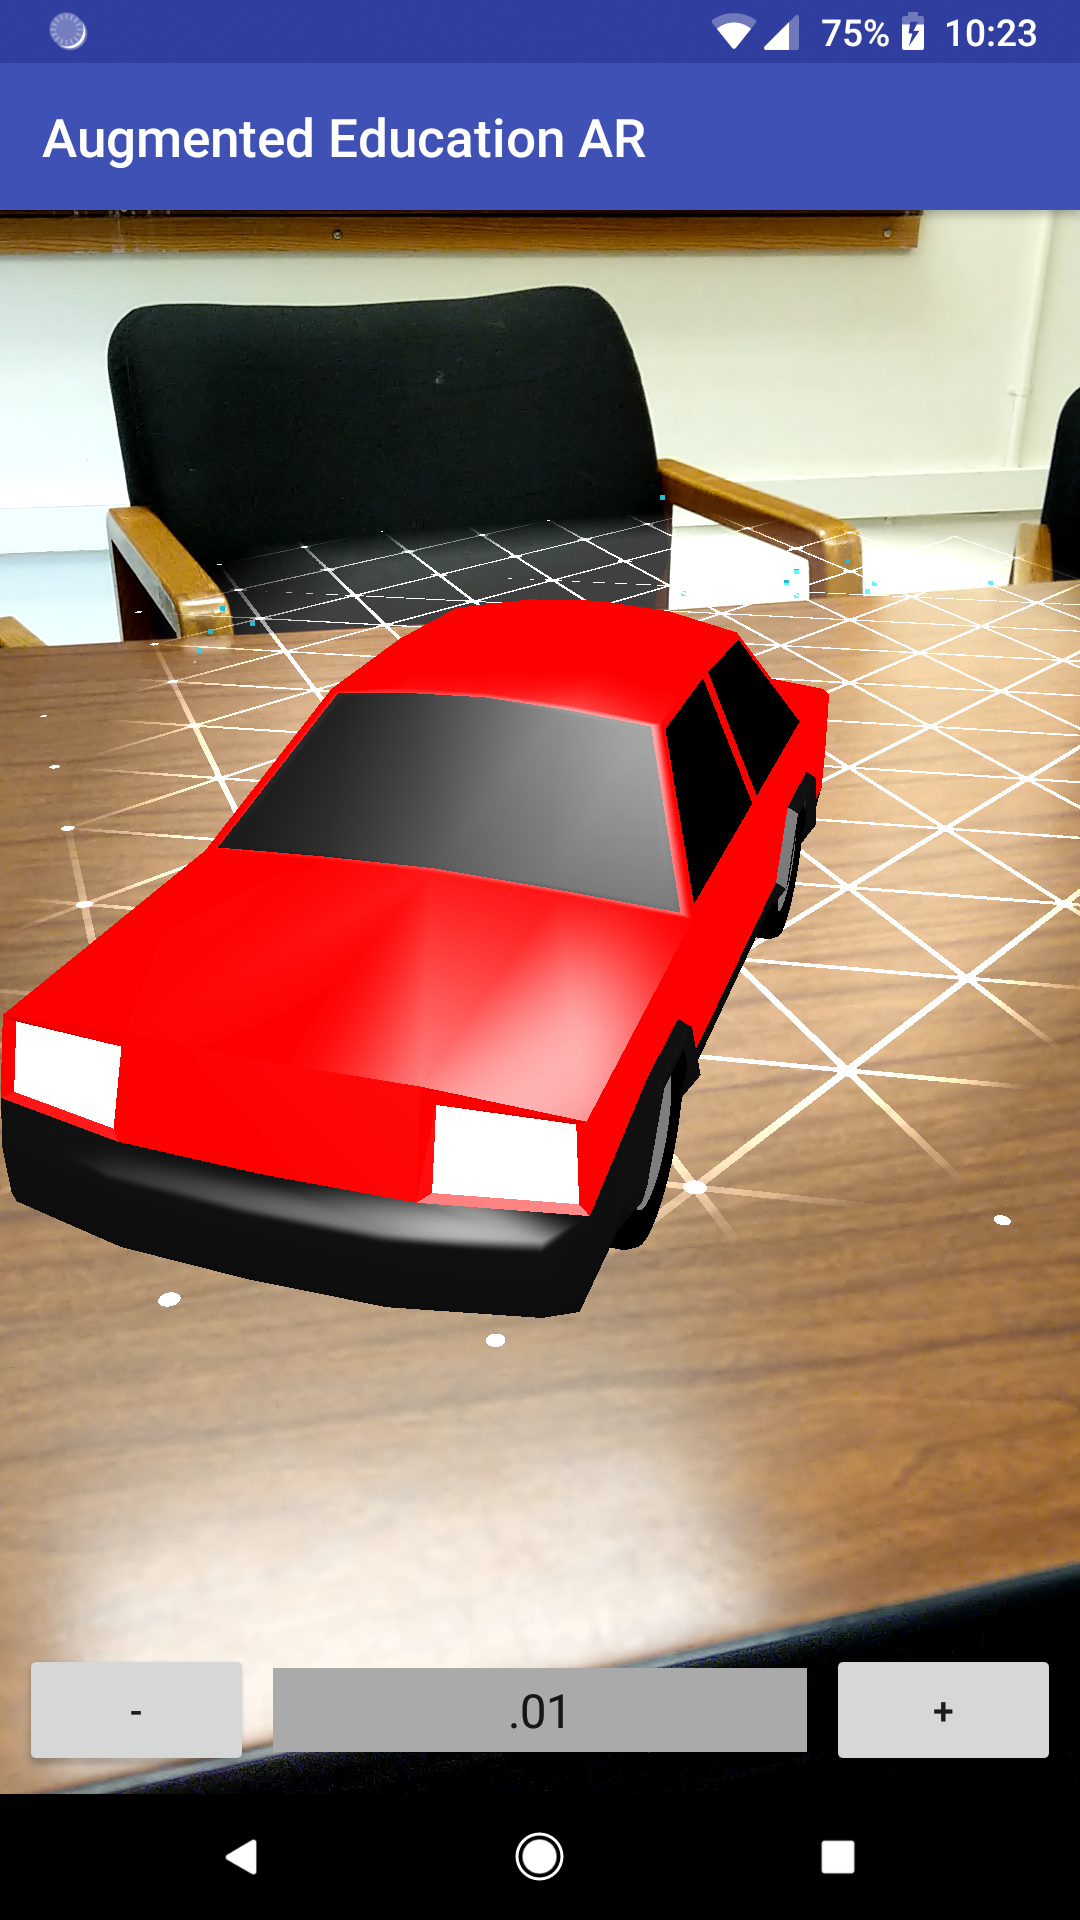
\includegraphics[width=0.5\textwidth]{Mobile/Mobile_Car}
                \centering
                \caption{Colors - Car}
                \label{fig:mobileCar}
            \end{figure}
        
        \subsubsection{Large Files}
        
            One main concern was that 3D files can get large and complex. The BMW is an example of this because it has 51,318 vertices while the sphere only has 2,258. It took a longer amount of time ($\sim$5 seconds) to load this file and it draws poorly, showing a limitation of keeping track of so many vertices.
            \begin{figure}[H]
                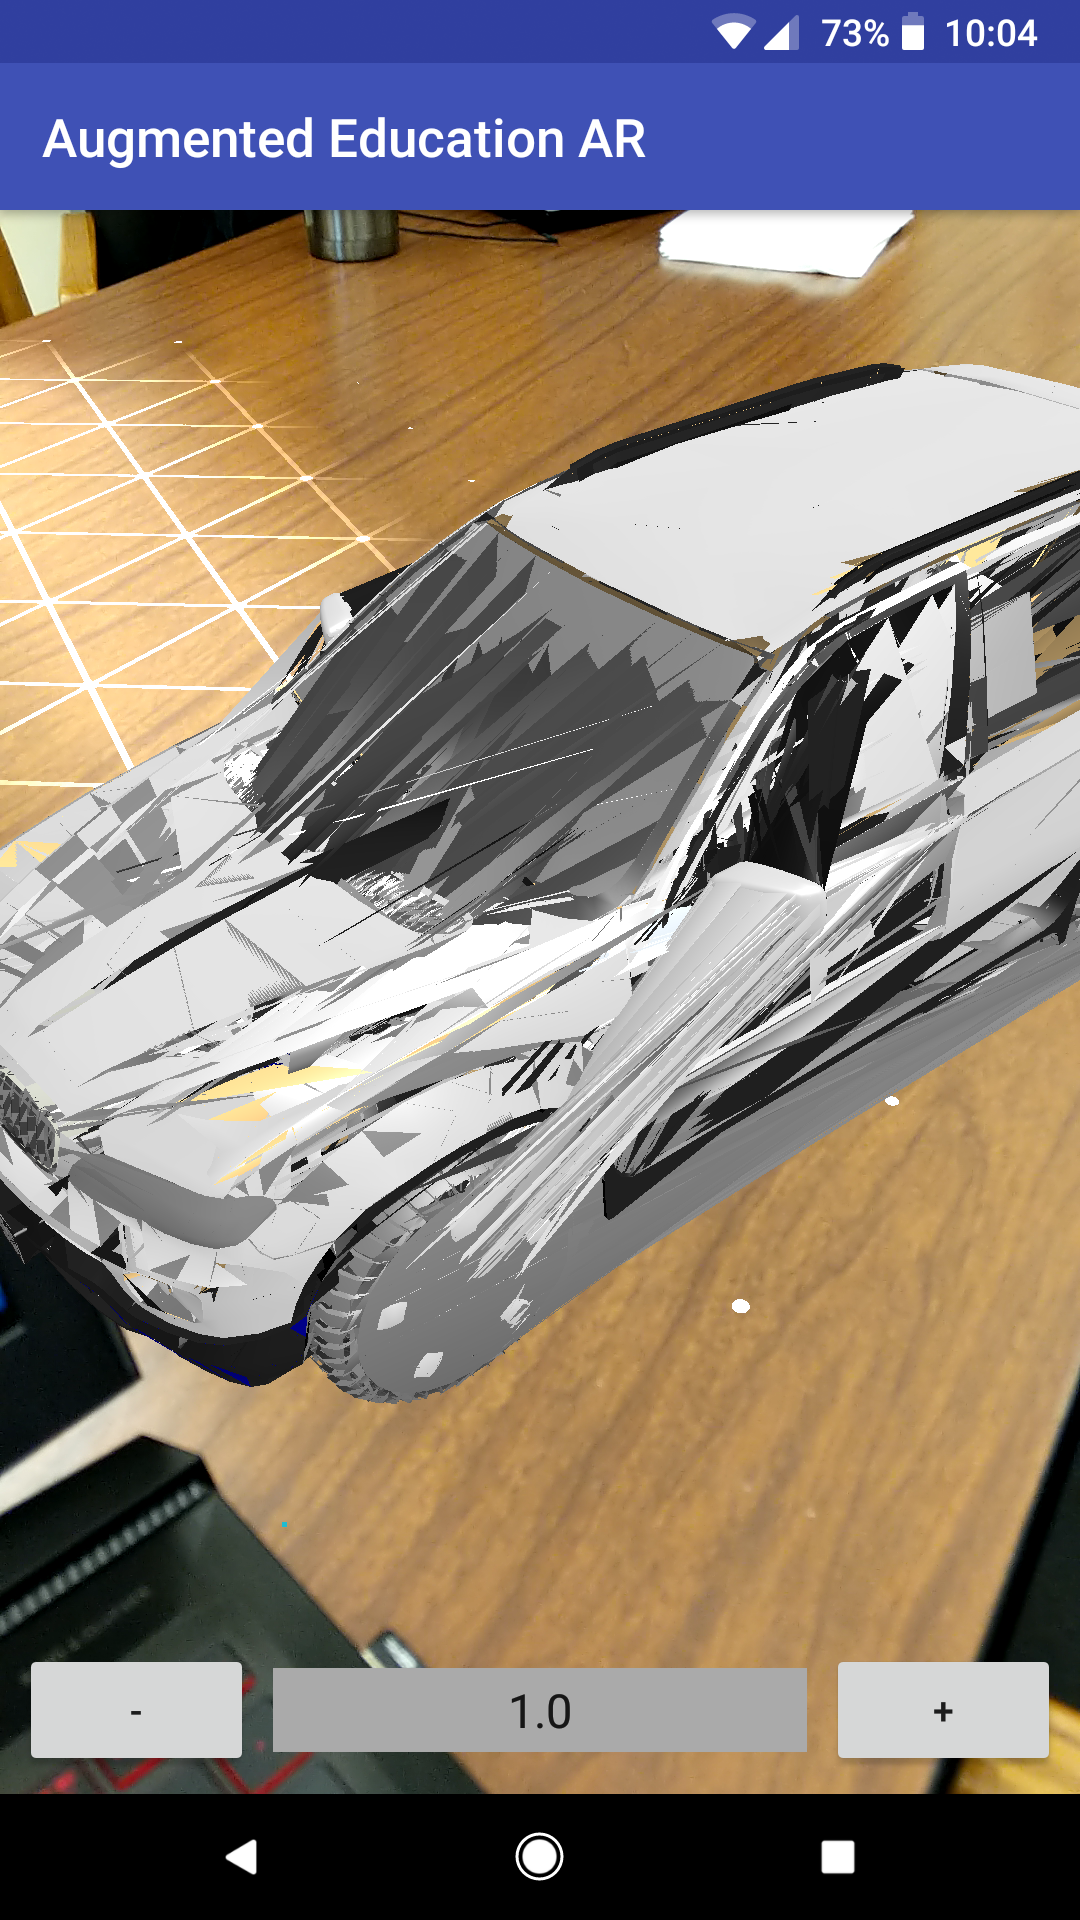
\includegraphics[width=0.5\textwidth]{Mobile/Mobile_BMW}
                \centering
                \caption{Large File - BMW}
                \label{fig:mobileBMW}
            \end{figure}
    
        \subsubsection{Small Files}
            A simple test used especially at the beginning of development to test that models would draw. The sphere is a typical example of something generated from Maple. 
        
            \begin{figure}[H]
                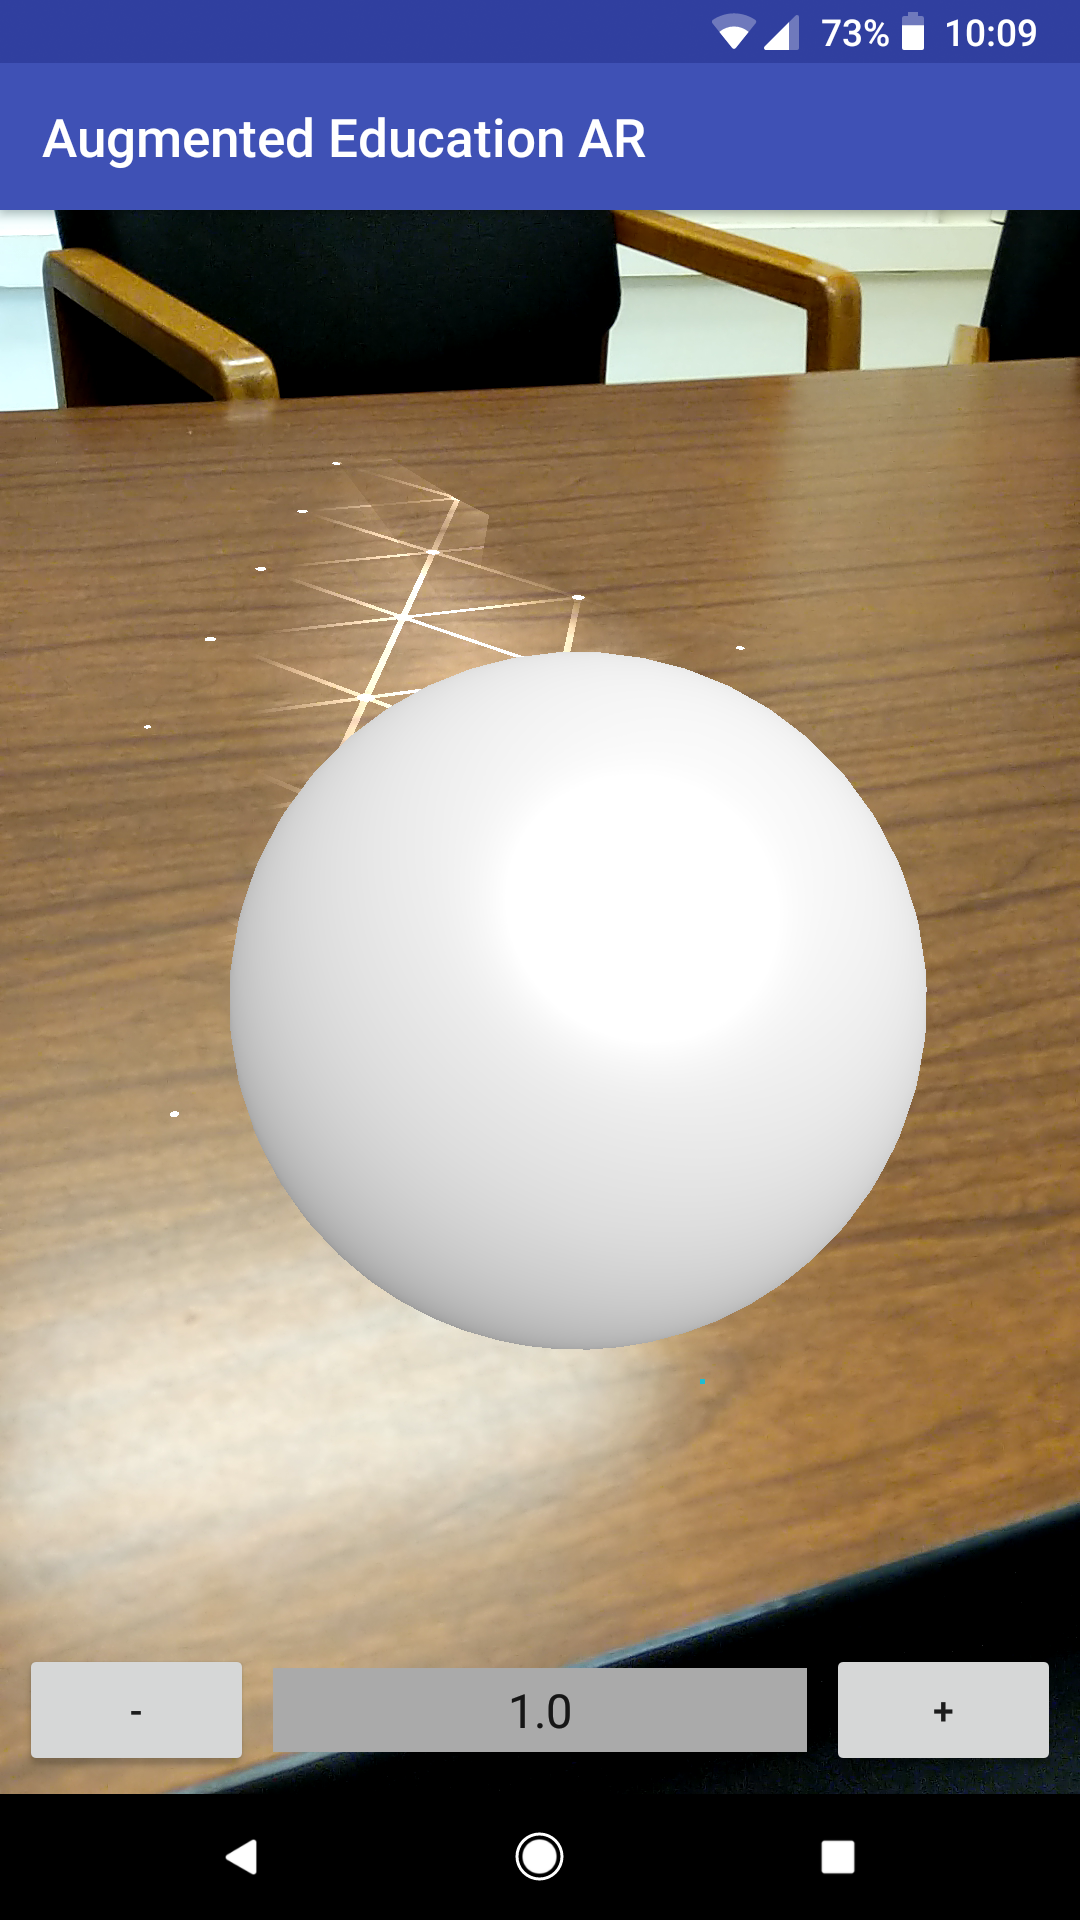
\includegraphics[width=0.5\textwidth]{Mobile/Mobile_Sphere}
                \centering
                \caption{Small File - Sphere}
                \label{fig:mobileSphere}
            \end{figure}
            
        \subsubsection{Embedded Images}
            
            Some 3D modeling software generates OBJ files with PNG textures referenced in the MTL instead of defining RGB values. It was necessary to test that these files were also supported by the app after adding extra functionality for them. Figure \ref{fig:mobileEmbeddedPhone} shows the PNG texture working, but it doesn't match the intended plot perfectly (Figure \ref{fig:mobileEmbeddedWindows}). This is because the app currently does not support drawing multiple images on top of each other yet.
        
            \begin{figure}[H]
                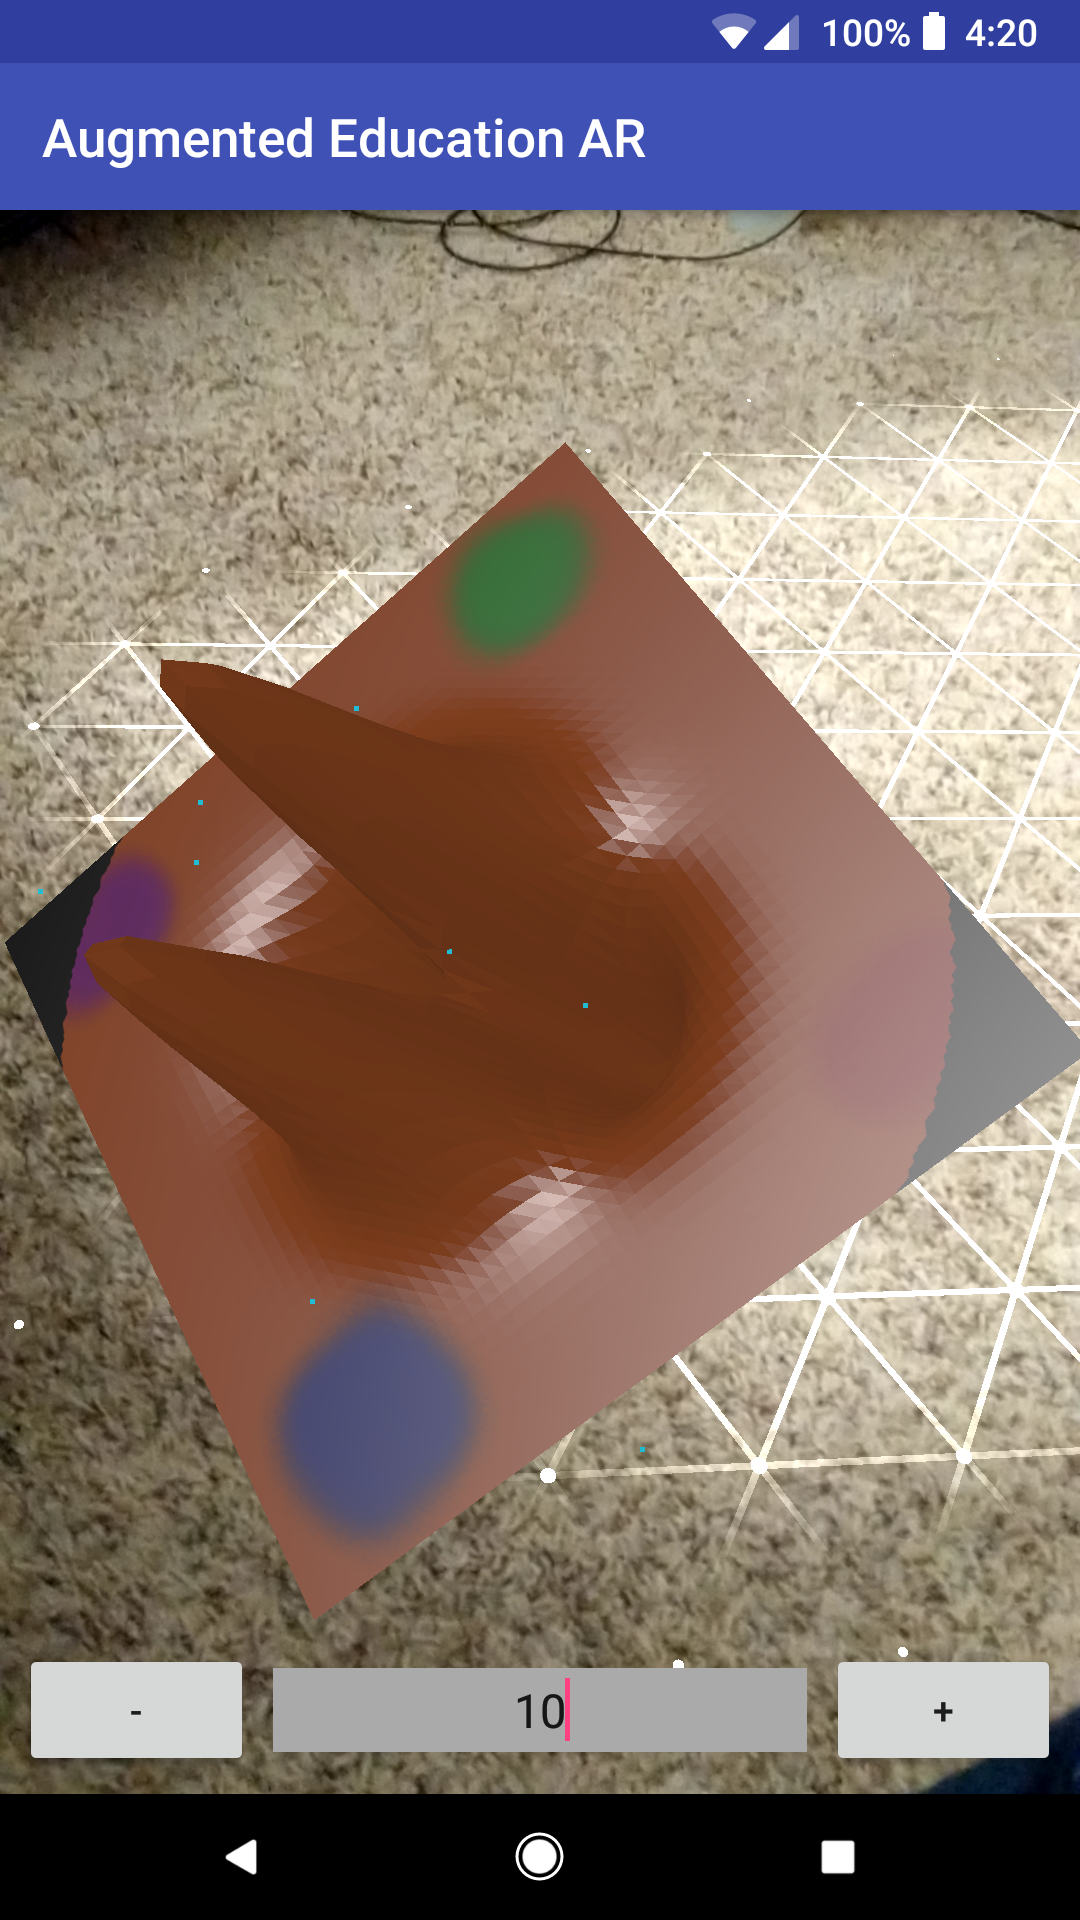
\includegraphics[width=0.5\textwidth]{Mobile/Mobile_ImagesPhone}
                \centering
                \caption{Embedded Image - Viewing on the phone}
                \label{fig:mobileEmbeddedPhone}
            \end{figure}

            \begin{figure}[H]
                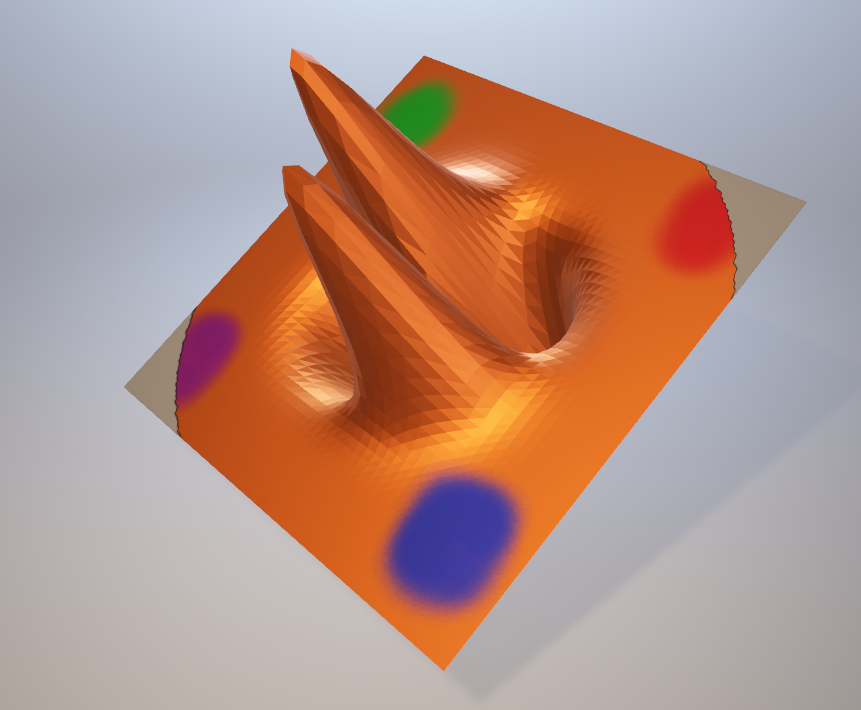
\includegraphics[width=0.5\textwidth]{Mobile/Mobile_ImagesWin}
                \centering
                \caption{Embedded Image - Viewing in the Windows Viewer}
                \label{fig:mobileEmbeddedWindows}
            \end{figure}

        \subsubsection{Scaling}

            Different models scale differently when initially drawn in the app. A scale factor of 1.0 on one model may be too small or too large, making the model difficult to visualize. To remedy this, the app provides an option to increase or decrease the scale factor, as well as change the step so models of different scales can be adjusted properly. Maple models generally need a larger scale factor (approx 3.0) while others like the car need to be adjusted by 0.1 at a time.
        
    \subsection{Web Interface}

        Another major component of the mobile app was the communication with the website.  If the app can display the models, there is little purpose if there is no method to get the models onto the phone.  The web API provided by the web team provides a method for communicating with the website.  It is done using the Volley library, provided by Google.  It abstracts the low level sending/receiving of networking communication away from the developer.  The code for these interfaces in primarily located in the \texttt{WebAccessor} Java class.

        Testing has shown that while the website is on Azure, the responsiveness is not always the best.  It is not infrequent to receive timeout errors on requests.  When this occurs, a message is displayed to the user.
        
        \subsubsection{Endpoints}\label{sec:Mobile_Auth}
        
            The endpoints used by the mobile application allow the app to: authenticate with the website, get a list of owned models, and download a model.  The endpoints were tested using Postman (to make sure the response was what was expected), the Android Studio debugger to make sure the correct fields were set, and a packet capture application to view the actual HTTP message sent from the phone.

            \paragraph{Authenticate}

                The authentication endpoint allowed the user to provide a username and password to get access to the website.  If the user entered valid credentials, an auth token is returned that allows the application to make requests on behalf of the user.  The auth token is used in the other API calls to the server.

                This API call is only performed on the Main Activity screen (the login page).  If a user is not authenticated, the user cannot continue through the app unless they select the Offline Mode button to not perform future web communication tasks.  A success of this component was, if the user supplied valid credentials, a valid auth token was returned.  Otherwise, an error message should be printed.  The testing was performed manually by trying invalid usernames/passwords.  In these cases, the website did not provide a valid auth token.  When correct usernames/passwords were entered, an auth token is returned.

                The Postman view that was used to test the endpoint (on the web side) is shown in Figure \ref{fig:mobilePostmanGetAuthToken}.

                \begin{figure}[H]
                    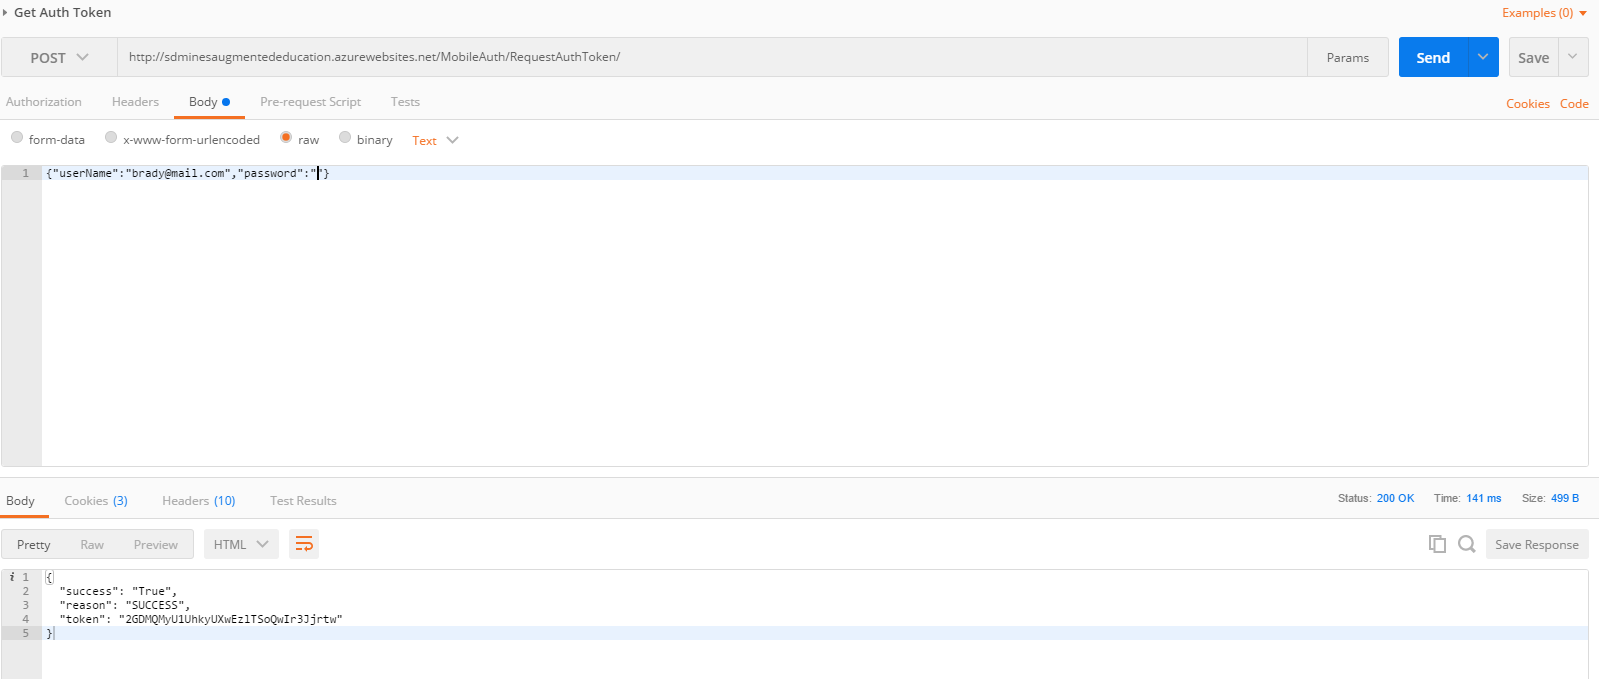
\includegraphics[width=0.75\textwidth]{postman_GetAuthToken}
                    \centering
                    \caption{Postman - Get authentication token}
                    \label{fig:mobilePostmanGetAuthToken}
                \end{figure}
                
            \paragraph{List Models}

                Another endpoint that is used by the mobile device is the one to get a listing of files owned by the user.  Like with the authentication token request, this call was tested manually to ensure the HTTP packets were well formed, and as expected.  Postman was again used to help test.  Figure \ref{fig:mobilePostmanListFiles} shows the Postman setup to send a request for a file listing.  
                
                \begin{figure}[H]
                    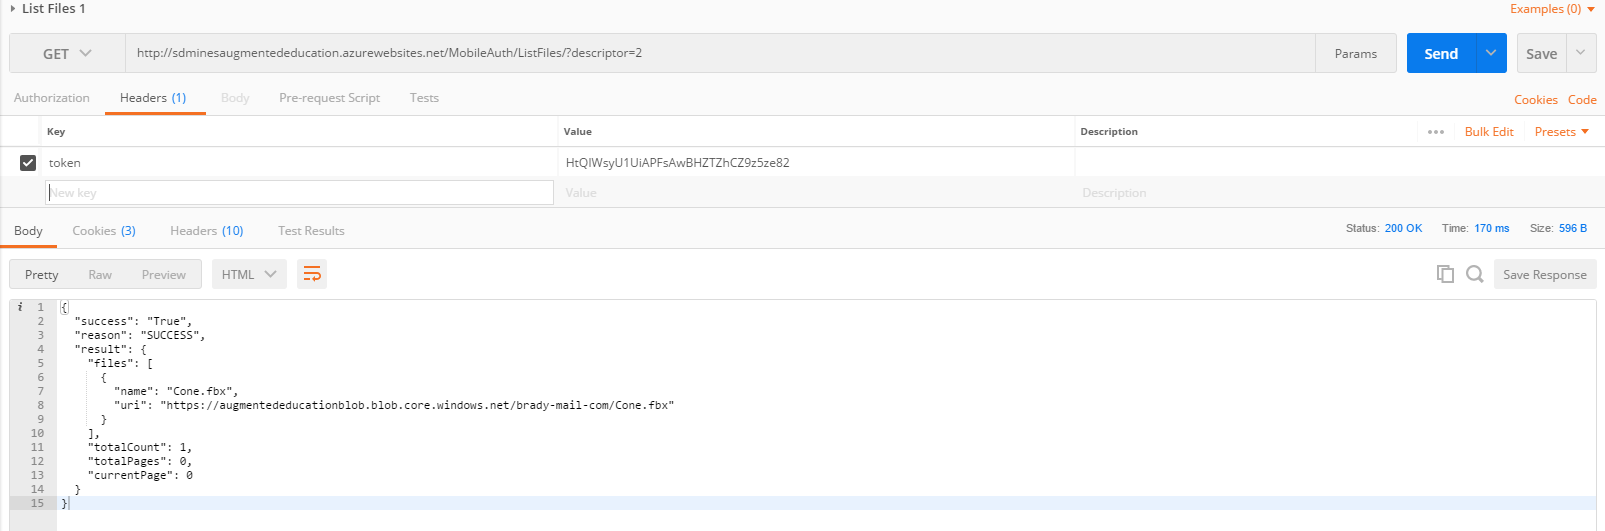
\includegraphics[width=0.75\textwidth]{postman_ListFiles}
                    \centering
                    \caption{Postman - List files}
                    \label{fig:mobilePostmanListFiles}
                \end{figure}
                
                Note, the \texttt{descriptor=} at the end of the URL, as it is used to state which files are desired for download.  An agreement was made between the mobile and web teams on what the levels should be.  There is an enumeration defined in the Java code with more details on the values and meanings.  Testing the different values showed a bug in the web code that always caused an error on the mobile device.  This issue was fixed by the web team.
            
            \paragraph{Download Model}

                Downloading a model includes contacting two endpoints.  One is used to get a temporary link to actually download the file, and the next downloads the file from that URL.  This is used so the phone can store the long term location, and get a temporary active URL to get the file.  Testing for these sections again included using Postman, and using a web browser to facilitate the download.  The Postman settings to get the temporary URL are located in Figure \ref{fig:mobilePostmanDownloadFile}.

                \begin{figure}[H]
                    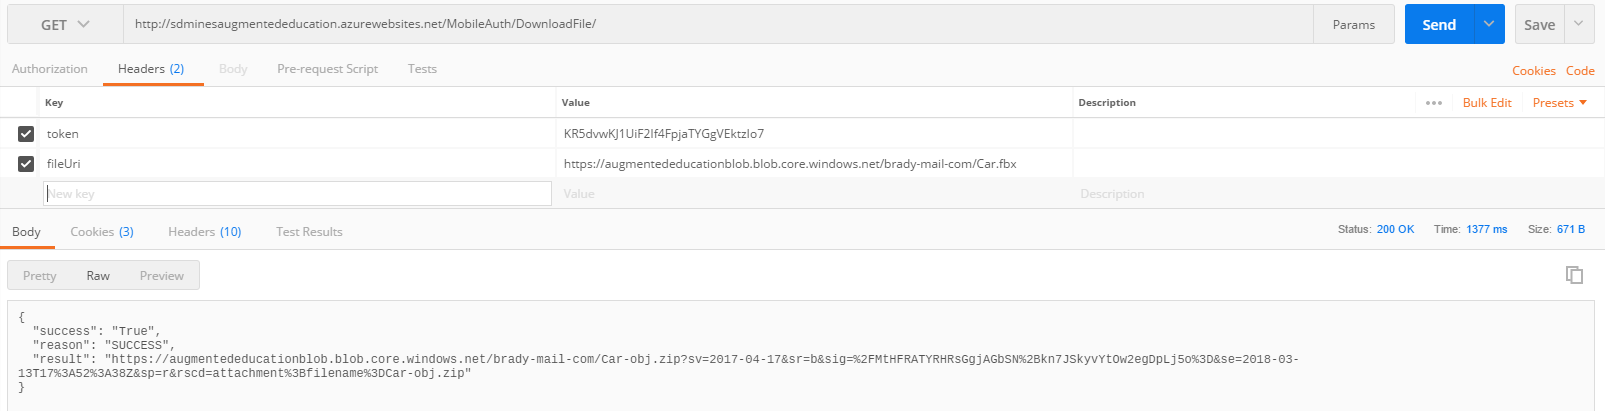
\includegraphics[width=0.75\textwidth]{postman_DownloadFile}
                    \centering
                    \caption{Postman - Download a file}
                    \label{fig:mobilePostmanDownloadFile}
                \end{figure}

                The field \texttt{result} contains the temporary URL.  It would then be put into a web browser (typically Firefox or Chrome) and the file is downloaded.  The file downloaded should be in the OBJ file format, since it is the one that is parse-able by the phone.  The website should use the file conversion software ensure this.  When the models are downloaded, they are stored in a \texttt{Models} directory on the phone.  The file system on the device can be viewed with the Downloads app.  Note, if the model is downloaded, and it does not show up in the file structure, the phone should be restarted.  Commonly, the files do not show up until the device is restarted.  A new folder will be created in the \texttt{Models} directory.  This is because one OBJ model can have multiple other models associated with it, including MTL (material) files and images.  When the models are downloaded, a zip archive is actually downloaded and extracted.

                Future developers should be aware of how the models are saved from the Android download manager.  When making the call for the download manager to do the download, a final path/file name must be provided.  This can cause issues if the file is saved with the wrong extension, especially if the files are viewed on the developers computer (and not just on the phone).
        
        \subsubsection{No Internet}

            Since internet can be less than reliable on cell phones, it was important to test if the there was no internet on the phone.  This was done by turning off Wifi on the testing phones (as they do not have cellular activated).  As expected, if there is no internet, an error message is displayed to the user that the communication was unsuccessful.
        
    \subsection{Offline Mode}
        
        When preparing for the Senior Design Fair, the mobile team decided that it would be a good idea to add an offline mode so the user can view models without having to authenticate with the server.  This was because the Wifi capabilities at the fair would be slim to none.  Therefore, an "Offline Mode" button was added to the login page to allow the user to continue offline.  Testing needed to be done on this to only show models registered as on the phone, as the user would not be able to download remote files without first authenticating.  This was tested and implemented in the application.  The application will not get a list of models from the website or download files from the website in offline mode.  The rest of the functionality (such as viewing the models) remained the same, which was as desired.

    \subsection{QR Code Scanning}
        
        To test that the app was scanning QR codes as expected during development, the team tried a number of different QR codes found online and printed on objects around. There were a surprising amount of these objects on hand with printed QR codes to test with. Testing on these gave an idea of the performance of the QR code scanner for varying QR code sizes.

        The scanner worked with QR codes that pointed to the 3D model downloads.  One difficulty of testing this was the way that the list of models was populated.  When the list was originally populated, all models owned by the user, and models that were public were added to the list.  So, all of the models that the user could access would already be in the list, so scanning a QR code would do nothing.  A later revision changed this so only privately owned files were added to the list, so QR codes can now usefully be scanned. Once the team had the functionality to embed the download link in a QR code, the team tested downloading a number of files manually using their respective QR codes.

    \subsection{Database}
        
        To test the database, the team primarily tested manually by using the test 3D model files. The database is populated by all the models private to the user's account. The team verified that when models are added to the user's account, the database is updated with a listing of the new models. The database also adds entries for scanned QR code files.